%%%%%%%%%%%%%%%%%%%%%%%%%%%%%%%%%%%%%%%%%
% HW Template
% LaTeX Template
% Version 1.0 (19/10/18)
% Modified by
% Erdem TUNA
% Halil TEMURTAŞ 
% Enes TAŞTAN 
%%%%%%%%%%%%%%%%%%%%%%%%%%%%%%%%%%%%%%%%%
%
%----------------------------------------------------------------------------------------
%	PACKAGES AND OTHER DOCUMENT CONFIGURATIONS
%----------------------------------------------------------------------------------------
\documentclass[a4paper,12pt]{article}
%-----packages------
\usepackage[a4paper, total={6.2in, 8.5in}]{geometry}
\usepackage[english]{babel}
\usepackage[utf8x]{inputenc}
\usepackage{amsmath}
\usepackage{mathtools}
\usepackage{graphicx}
\usepackage[colorinlistoftodos]{todonotes}
\usepackage{gensymb} % this could be problem
\usepackage{float}
\usepackage{fancyref}
\usepackage{subcaption}
\usepackage[toc,page]{appendix} %appendix package
\usepackage{xcolor}
\usepackage{listings}
\usepackage{xspace}
\usepackage{amssymb}
\usepackage{nicefrac}
\usepackage{gensymb}
\usepackage{fancyhdr}
\usepackage{blindtext}  % for dummy text, use \blindtext or \BlindText
\usepackage{lipsum}    % for dummy text, use \lipsum[3-56]
\usepackage[final]{pdfpages}  % pdf include
\usepackage{array} %allows more options in tables
\usepackage{pgfplots,pgf,tikz} %coding plots in latex
\usepackage{capt-of} % allows caption outside the figure environment
\usepackage[export]{adjustbox} %more options for adjusting the images
\usepackage{multicol,multirow,slashbox} % allows tables like table1
%\usepackage[hyperfootnotes=false]{hyperref} % clickable references
\usepackage{epstopdf} % useful when matlab is involved
%\usepackage{placeins} % prevents the text after figure to go above figure with \FloatBarrier 
%\usepackage{listingsutf8,mcode} %import .m or any other code file mcode is for matlab highlighting

%-----end of packages

%-----specifications-----
\definecolor{mGreen}{rgb}{0,0.6,0} % for python
\definecolor{mGray}{rgb}{0.5,0.5,0.5}
\definecolor{mPurple}{rgb}{0.58,0,0.82}
\definecolor{mygreen}{RGB}{28,172,0} % color values Red, Green, Blue for matlab
\definecolor{mylilas}{RGB}{170,55,241}

\setcounter{secnumdepth}{5} % how many sectioning levels to assign numbers to
\setcounter{tocdepth}{5}    % how many sectioning levels to show in ToC

\lstdefinestyle{CStyle}{
	commentstyle=\color{mGreen},
	keywordstyle=\color{magenta},
	numberstyle=\tiny\color{mGray},
	stringstyle=\color{mPurple},
	basicstyle=\footnotesize,
	breakatwhitespace=false,         
	breaklines=true,
	frame=single,
	rulecolor=\color{black!40},                 
	captionpos=b,                    
	keepspaces=true,                 
	numbers=left,                    
	numbersep=5pt,                  
	showspaces=false,                
	showstringspaces=false,
	showtabs=false,                  
	tabsize=2,
	language=C
}

\lstset{language=Matlab,%
	%basicstyle=\color{red},
	breaklines=true,%
	frame=single,
	rulecolor=\color{black!40},
	morekeywords={matlab2tikz},
	keywordstyle=\color{blue},%
	morekeywords=[2]{1}, keywordstyle=[2]{\color{black}},
	identifierstyle=\color{black},%
	stringstyle=\color{mylilas},
	commentstyle=\color{mygreen},%
	showstringspaces=false,%without this there will be a symbol in the places where there is a space
	numbers=left,%
	numberstyle={\tiny \color{black}},% size of the numbers
	numbersep=9pt, % this defines how far the numbers are from the text
	emph=[1]{for,end,break},emphstyle=[1]\color{red}, %some words to emphasise
	%emph=[2]{word1,word2}, emphstyle=[2]{style},    
}


\tikzset{
	desicion/.style={
		diamond,
		draw,
		text width=4em,
		text badly centered,
		inner sep=0pt
	},
	block/.style={
		rectangle,
		draw,
		text width=10em,
		text centered,
		rounded corners
	},
	cloud/.style={
		draw,
		ellipse,
		minimum height=2em
	},
	descr/.style={
		fill=white,
		inner sep=2.5pt
	},
	connector/.style={
		-latex,
		font=\scriptsize
	},
	rectangle connector/.style={
		connector,
		to path={(\tikztostart) -- ++(#1,0pt) \tikztonodes |- (\tikztotarget) },
		pos=0.5
	},
	rectangle connector/.default=-2cm,
	straight connector/.style={
		connector,
		to path=--(\tikztotarget) \tikztonodes
	}
}

\tikzset{
	desicion/.style={
		diamond,
		draw,
		text width=4em,
		text badly centered,
		inner sep=0pt
	},
	block/.style={
		rectangle,
		draw,
		text width=10em,
		text centered,
		rounded corners
	},
	cloud/.style={
		draw,
		ellipse,
		minimum height=2em
	},
	descr/.style={
		fill=white,
		inner sep=2.5pt
	},
	connector/.style={
		-latex,
		font=\scriptsize
	},
	rectangle connector/.style={
		connector,
		to path={(\tikztostart) -- ++(#1,0pt) \tikztonodes |- (\tikztotarget) },
		pos=0.5
	},
	rectangle connector/.default=-2cm,
	straight connector/.style={
		connector,
		to path=--(\tikztotarget) \tikztonodes
	}
}
%-----end of specifications-----


%----commands----
\newcommand\nd{\textsuperscript{nd}\xspace}
\newcommand\rd{\textsuperscript{rd}\xspace}
\newcommand\nth{\textsuperscript{th}\xspace} %\th is taken already
\newcommand{\specialcell}[2][c]{ \begin{tabular}[#1]{@{}c@{}}#2\end{tabular}} % for too long table lines

\newcommand{\blankpage}{
	\- \\[9cm]	
	{ \centering \textit{This page intentionally left blank.} \par }
	\- \\[9cm]
}% For Blank Page

\makeatletter
\renewcommand\paragraph{\@startsection{paragraph}{4}{\z@}%
	{-2.5ex\@plus -1ex \@minus -.25ex}%
	{1.25ex \@plus .25ex}%
	{\normalfont\normalsize\bfseries}}
\makeatother
%-----end of commands-----


\pagestyle{fancy}
\fancyhead[LO,LE]{Halil TEMURTAŞ / 2094522   }
\fancyhead[RO,RE]{November 23,2018}
\fancyfoot[RO,RE]{
\includegraphics[width=2.7cm]{images/eelogo}}

\begin{document}
\begin{center}
	\textbf{\large EE402 Discrete Time Systems \\[0.2cm] MP-3} \\
\end{center}


\begin{enumerate}
	\item Let us define;
	\begin{equation*}
		\begin{split}	
		 G_1(s) &=  \frac{s}{s^2-1} 	\\
		 G_2(s) &= \frac{1}{s} \\
		 G_{ZOH}(s) &= \frac{1-z^{-1}}{s} \\
		 G_X(s) &= G_{ZOH}(s) G_1(s)  \\[0.3cm] 
		 G_Y(s) &= G_{ZOH}(s)G_1(s) G_2(s)	
		\end{split}
	\end{equation*}
		
		
	
	
	\begin{figure}[H]
			\center
			\setlength{\unitlength}{\textwidth} 
		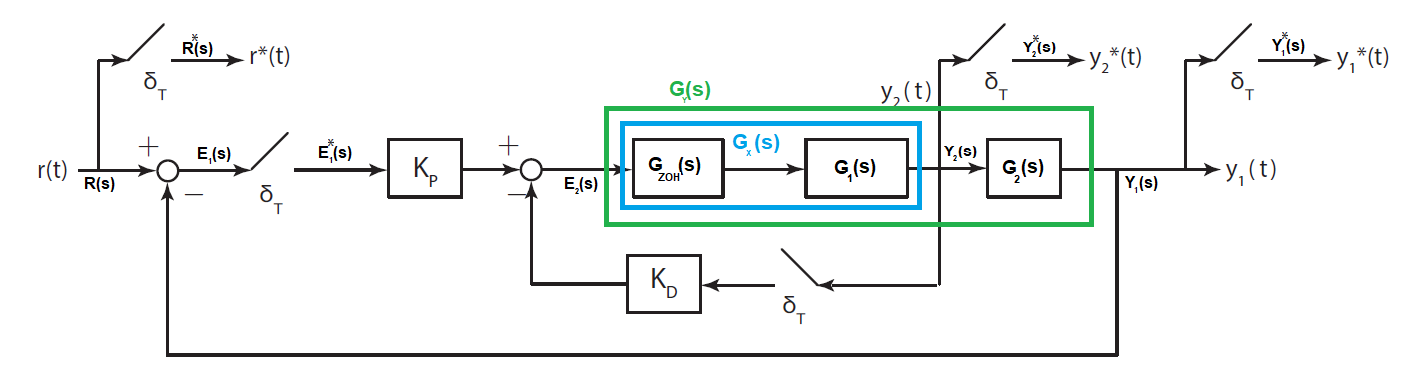
\includegraphics[width=1.0\unitlength]{images/q1o}
  		\caption{\label{fig:q1m}Block Diagram Representation of the System}
	\end{figure}
	
	\begin{enumerate}
		\item 
		
		\begin{equation*}
		\begin{split}		
		 E(s) &= R(s) - Y_1(s)  \\
		 E^*(s) &= R^*(s) - Y_1^*(s) \\[0.3cm]		 
		 Y_1(s) &= E^*(s) K_p G_Y(s)  \\
		 Y_1^*(s) &= E^*(s) K_p G_Y^*(s) \\[0.3cm]
		 \frac{Y_1^*(s)}{R^*(s)}&=K_pG_Y^*(s)\\[0.3cm]				 
		 E^*(s) &= R^*(s) - E^*(s) K_p G_Y^*(s) \\[0.3cm]
		 \frac{E^*(s)}{R^*(s)}&=\frac{1}{1+K_pG_Y^*(s)} \\[0.3cm]	  
		 \frac{Y_1^*(s)}{R^*(s)} &= \frac{E^*(s)}{R^*(s)} \ \frac{Y_1^*(s)}{E^*(s)} = \frac{K_p G_Y^*(s)}{1+K_pG_Y^*(s)} 
		\end{split}
		\end{equation*}
		

		Thus, with $s=\frac{1}{T}ln(z)$
		$$\boxed{ \frac{Y_1(z)}{R(z)} = \frac{K_p G_Y(z)}{1+K_pG_Y(z)} }$$
		
		$$ 	Y_2(s) = E^*(s) K_p G_X(s)  $$
		$$  Y_2^*(s) = E^*(s) K_p G_X^*(s) $$
		
		$$ \frac{Y_2^*(s)}{R^*(s)} = \frac{E^*(s)}{R^*(s)} \ \frac{Y_2^*(s)}{E^*(s)} = \frac{K_p G_X^*(s)}{1+K_pG_Y^*(s)}  $$
		
		Thus, with $s=\frac{1}{T}ln(z)$
		$$\boxed{ \frac{Y_2(z)}{R(z)} = \frac{K_p G_X(z)}{1+K_pG_Y(z)} }$$
		
		
		%%%%%%%%%%%%%%%%%%%%%%%%%%%
		
		\newpage
		
		Let us now find $G_X(z)$ and $G_Y(s)$ to find the pulse transfer functions,
		
		$$ G_Y(z)=\mathcal{Z}\{G_Y(s)\}  =\mathcal{Z}\{ {\mathcal{L}^{-1}\{G_{ZOH}(s)G_1(s)G_2(s)\}}^*	\}$$
		with $G_{ZOH}(s)=\dfrac{1-e^{-Ts}}{s}$ and $G_1(s)G_2(s)=\dfrac{1}{s^2-1}$ and $\boxed{T=0.5}$
		
			$$\boxed { G_Y(z)=\left((1-z^{-1}) \mathcal{Z}\{ \frac{G_1(s)G_2(s)}{s} \}\right) }$$ 
			\begin{equation*}
				\begin{split}\\[-0.3cm]  \hline \\[-0.3cm] 
		 			\mathcal{Z}\left\{ \frac{G_1(s)G_2(s)}{s} \right\}&=\mathcal{Z}\left\{ \frac{1}{s(s^2-1)} \right\} \\
					&= \mathcal{Z} \left\{ \frac{-1}{s}+\frac{1}{2(s+1)}+\frac{1}{2(s-1)} \right\}\\
					&=\frac{-1}{1-z^{-1}}+ \frac{1}{2(1-e^{0.5}z^{-1})}+ \frac{1}{2(1-e^{-0.5}z^{-1})} \\[0.3cm]  \hline 
					\\[-0.3cm] 
					G_Y(z)&=-1+ \frac{1-z^{-1}}{2(1-e^{0.5}z^{-1})}+ \frac{1-z^{-1}}{2(1-e^{-0.5}z^{-1})} \\[0.3cm]
					&=\frac{-2(1-e^{0.5}z^{-1})(1-e^{-0.5}z^{-1})+(1-z^{-1})(1-e^{-0.5}z^{-1})}{2(1-e^{0.5}z^{-1})(1-e^{-0.5}z^{-1})} \\[0.3cm]
					& +\frac{(1-z^{-1})(1-e^{0.5}z^{-1})}{2(1-e^{0.5}z^{-1})(1-e^{-0.5}z^{-1})} \\[0.3cm]
					G_Y(z)&=\frac{(e^{0.5}+e^{-0.5}-2)z^{-1}+(e^{0.5}+e^{-0.5}-2)z^{-2}}{2(1-(e^{0.5}+e^{-0.5})z^{-1}+z^{-2})} 
					\\[0.3cm]  \hline \\[-0.3cm]
					G_Y(z)&=\frac{\left[e^{0.5}+e^{-0.5}-2\right](z^{-1}+z^{-2})}{2(1-(e^{0.5}+e^{-0.5})z^{-1}+z^{-2})}  \\
					G_Y(z)&\approx \frac{0.255(z^{-1}+z^{-2})}{2(1-2.255z^{-1}+z^{-2})}
					\\[0.3cm]  \hline \\[-0.3cm]
				\end{split} 
			\end{equation*}
			
				$$\boxed  { G_Y(z)\approx \frac{0.1275(z+1)}{z^2-2.255z+1} }$$
				
				
			\newpage
			
			$$ \boxed  { G_X(z)=\left((1-z^{-1}) \mathcal{Z}\{ \frac{G_1(s)}{s} \}\right) }$$  
			\begin{equation*}
				\begin{split}\\[-0.3cm]  \hline \\[-0.3cm] 
					\mathcal{Z}\left\{ \frac{G_1(s)}{s} \right\}&=\mathcal{Z}\left\{ \frac{1}{s^2-1} \right\} \\[0.3cm]
					&= \mathcal{Z} \left\{ \frac{1/2}{s-1}-\frac{1/2}{s+1} \right\} \\[0.3cm]
					&= \frac{1/2}{1-e^{0.5}z^{-1}} - \frac{1/2}{1-e^{-0.5}z^{-1}}  =  \frac{\left[e^{0.5}-e^{-0.5}\right] z^{-1}}{2(1-e^{0.5}z^{-1})(1-e^{-0.5}z^{-1})} \\[0.3cm]
					&=  \frac{\left[e^{0.5}-e^{-0.5}\right] z^{-1}}{2(1-\left[ e^{0.5}+e^{-0.5} \right]z^{-1}+z^{-2} )}   
					\\[0.3cm]  \hline \\[-0.3cm]
					G_X(z)&= \frac{\left[e^{0.5}-e^{-0.5}\right] z^{-1} \left(1-z^{-1} \right) }{2(1-\left[ e^{0.5}+e^{-0.5} \right]z^{-1}+z^{-2} )}   \\[0.3cm]
					&= \frac{\left[e^{0.5}-e^{-0.5}\right]  \left(z^{-1}-z^{-2} \right) }{2(1-\left[ e^{0.5}+e^{-0.5} \right]z^{-1}+z^{-2} )} \\[0.3cm]
					&= \frac{\left[e^{0.5}-e^{-0.5}\right]  \left(z-1 \right) }{2(z^2-\left[ e^{0.5}+e^{-0.5} \right]z+1 )}
					\\[0.3cm]  \hline \\[-0.3cm]
			 	\end{split} 
			\end{equation*}
			
				$$\boxed  { G_X(z)\approx \frac{0.52  \left(z-1 \right) }{z^2-2.255z+1 } }$$
				
			\newpage
			
			Let us now put what we have found into pulse transfer function form.
				
			\begin{equation*}
				\begin{split}	
					 \frac{Y_1(z)}{R(z)} &= \frac{K_p G_Y(z)}{1+K_pG_Y(z)} \\
					 & = \cfrac{K_p \left(\cfrac{0.1275(z+1)}{z^2-2.255z+1}\right)}{1+K_p\left(\cfrac{0.1275(z+1)}{z^2-2.255z+1}\right)} \\
					 & = { \frac{0.1275K_p(z+1)}{z^2-2.255z+1+K_p(0.1275(z+1))} }
				\end{split}
			\end{equation*} 
			
			$$\boxed{\frac{Y_1(z)}{R(z)} =  \frac{0.1275K_p(z+1)}{z^2+(0.1275K_p-2.255)z+(1+1.0275K_p) }}  $$	
				
			\begin{equation*}
				\begin{split}	
					\frac{Y_2(z)}{R(z)} &= \frac{K_p G_X(z)}{1+K_pG_Y(z)} \\
					& = \cfrac{K_p \left(\cfrac{0.52  \left(z-1 \right)}{z^2-2.255z+1 }\right)}{1+K_p\left(\cfrac{0.1275(z+1)}{z^2-2.255z+1}\right)} \\
					&=\frac{0.52 K_p(z-1 )}{z^2-2.255z+1+1.0275K_p(z+1)}
				\end{split} 
			\end{equation*} 
			
			$$\boxed{\frac{Y_2(z)}{R(z)} =   \frac{0.52 K_p1(z-1 )}{z^2+(0.1275K_p-2.255)z+(1+0.1275K_p) } }   $$	
			
			
			\newpage
		
		
		
		\item To ensure stability conditions for $K_p$, Let us use Jury Conditions;
		$$ D(s)= z^2+(0.1275K_p-2.255)z+(1+0.1275K_p) $$
		With coefficients, 
		$$ \boxed{a_0=1} \ , \ \boxed{a_1=0.1275K_p-2.255} \ ,\ \boxed{a_2=1+0.1275K_p} $$		
		The characteristic polynomial $D(s)$ should satisfy the following conditions according to Jury stability conditions;
		\begin{itemize}
			\item $a_0\ >\ |a_2| $ \\
				$$ 1\ >\ 1+0.1275K_p > -1 $$
				$$\boxed{ 0 > K_p > -7.843 }$$
			\item $D(1)>0$ \\
				$$ 1+0.1275K_p-2.255+1+0.1275K_p > 0$$
				$$ 0.255K_p-1.1275>0$$
				$$ \boxed{ K_p>5.01} $$
			\item $D(-1)>0$ \\
				$$ 1-0.1275K_p+2.255+1+0.1275K_p > 0$$
				$$\boxed{ 2.1275>0 }$$				
		\end{itemize}
		It can be concluded that there are no $K_p$ value that makes the system stable.
		
		
 		\item Given that $K_p=2$, the unit step response can be calculated as follows;
 		
 		$$ R(z)= \frac{1}{1-z^{-1}}=\frac{z}{z-1}  $$
 		
 		\begin{equation*}
 			\begin{split}
	 			Y_1(z) &=  \frac{0.1275K_p(z+1)}{z^2-2.255z+1+0.1275K_p(z+1)} R(z)  \\	
 				&=  \frac{0.255(z^2+z)}{(z^2-2z+1.255)(z-1)} \\ 
 			\end{split}
 		\end{equation*}
 		
 		$$\boxed{Y_1(z) =   \frac{2.255(z^2+z)}{(z^2+3.255)(z-1)}  }  $$	
 		
		$$\boxed{  y_1[k] = \mathcal{Z}^{-1} \{Y_1(z)	\} } $$
		
 		
 		\begin{equation*}
 		\begin{split}
 		Y_2(z) &=   \frac{0.52 K_p(z-1 )}{z^2+(0.1275K_p-2.255)z+(1+0.1275K_p) }R(z) \\	
 		&=  \frac{1.04z(z-1)}{(z^2-2z+1.255)(z-1)} \\ 
 		&= \frac{1.04z}{z^2+-2z+1.255}
 		\end{split}
 		\end{equation*}
 		
 		$$\boxed{Y_2(z) =   \frac{1.04z}{z^2-2z+1.255} }  $$
 		
 		
 				
 		$$\boxed{ y_2(t) = \mathcal{Z}^{-1} \{Y_2(z)	\} }$$
 		
 		
 		\item The \textit{Figure\ \ref{fig:stepy1a}} shows the step responses of $y_1(t)$ and $y_2(t)$ for $k_{final}=50$ and $k_{final}=100$.  The source code for that operation can be seen at \textbf{Appendix~\ref{appendix}}.
 		
 		
 			
 			\begin{figure}[H]
 				\center
 				\setlength{\unitlength}{\textwidth} 
 				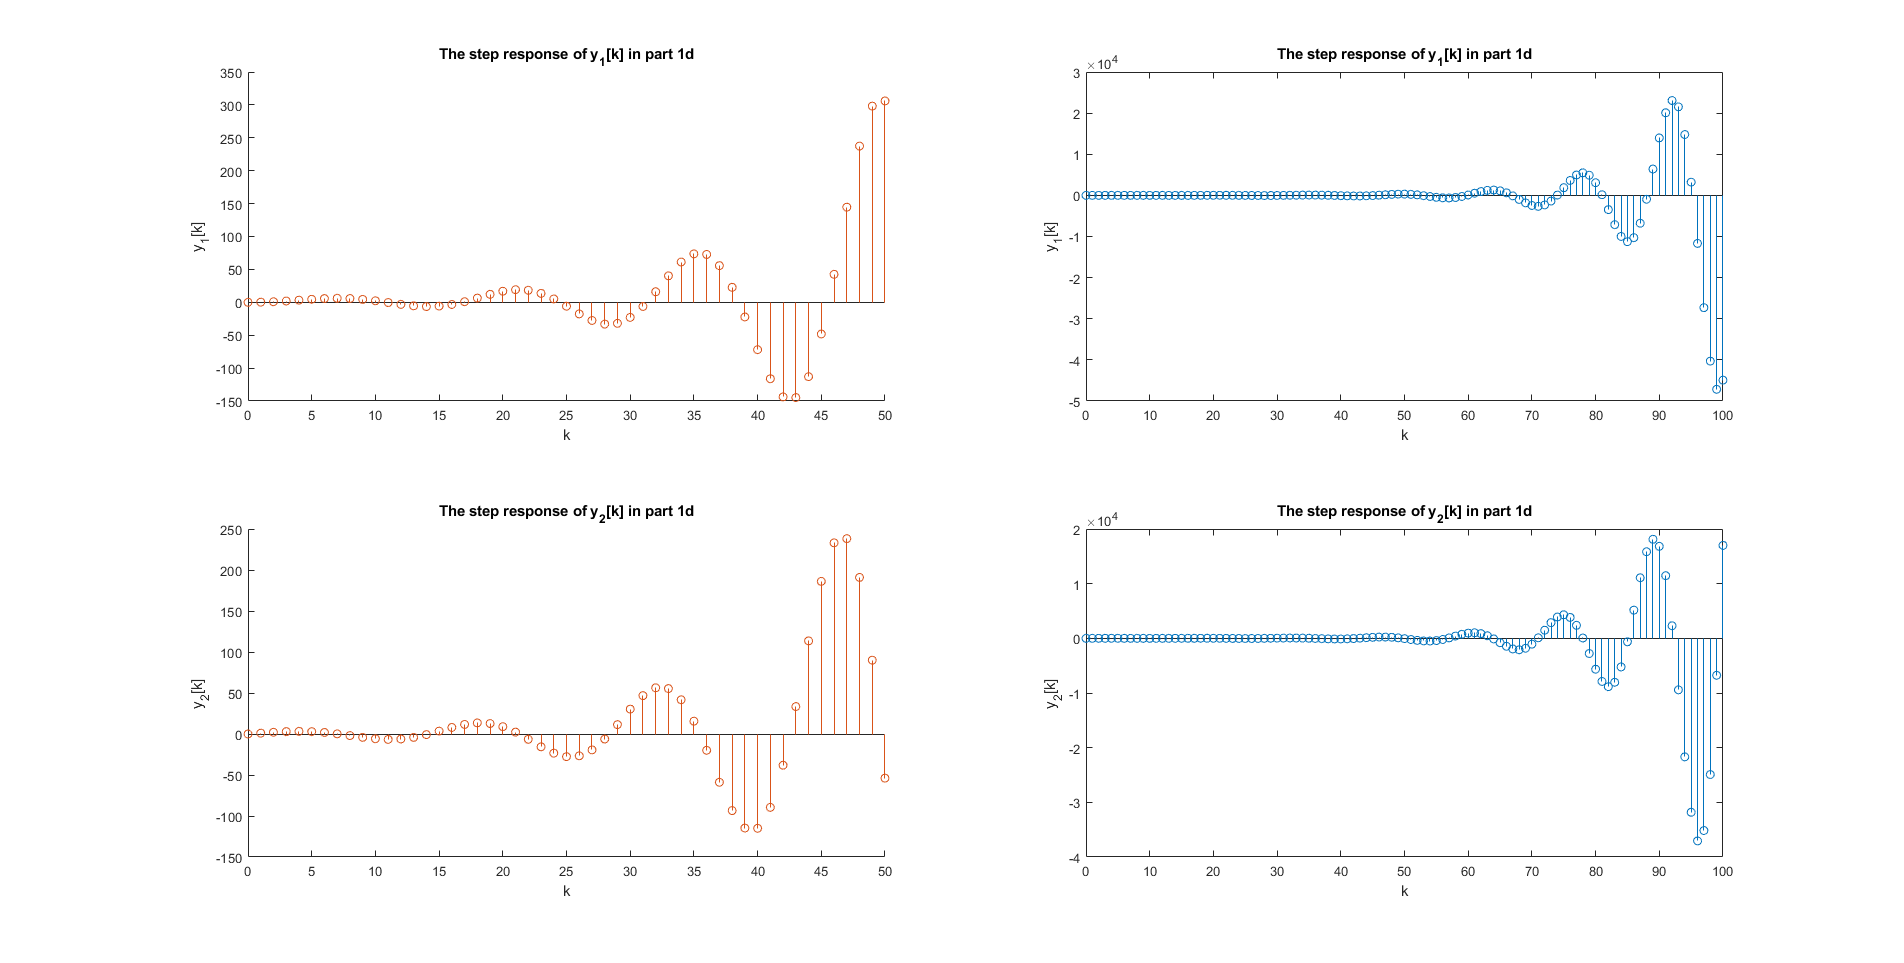
\includegraphics[width=1.0\unitlength]{images/1d}
 				\caption{\label{fig:stepy1a} Step Response for the $y_1(t)$ with $K_P=2$ and $K_D=0$}
 			\end{figure}
 		
 		
 			\begin{figure}[H]
 				\center
 				\setlength{\unitlength}{\textwidth} 
 				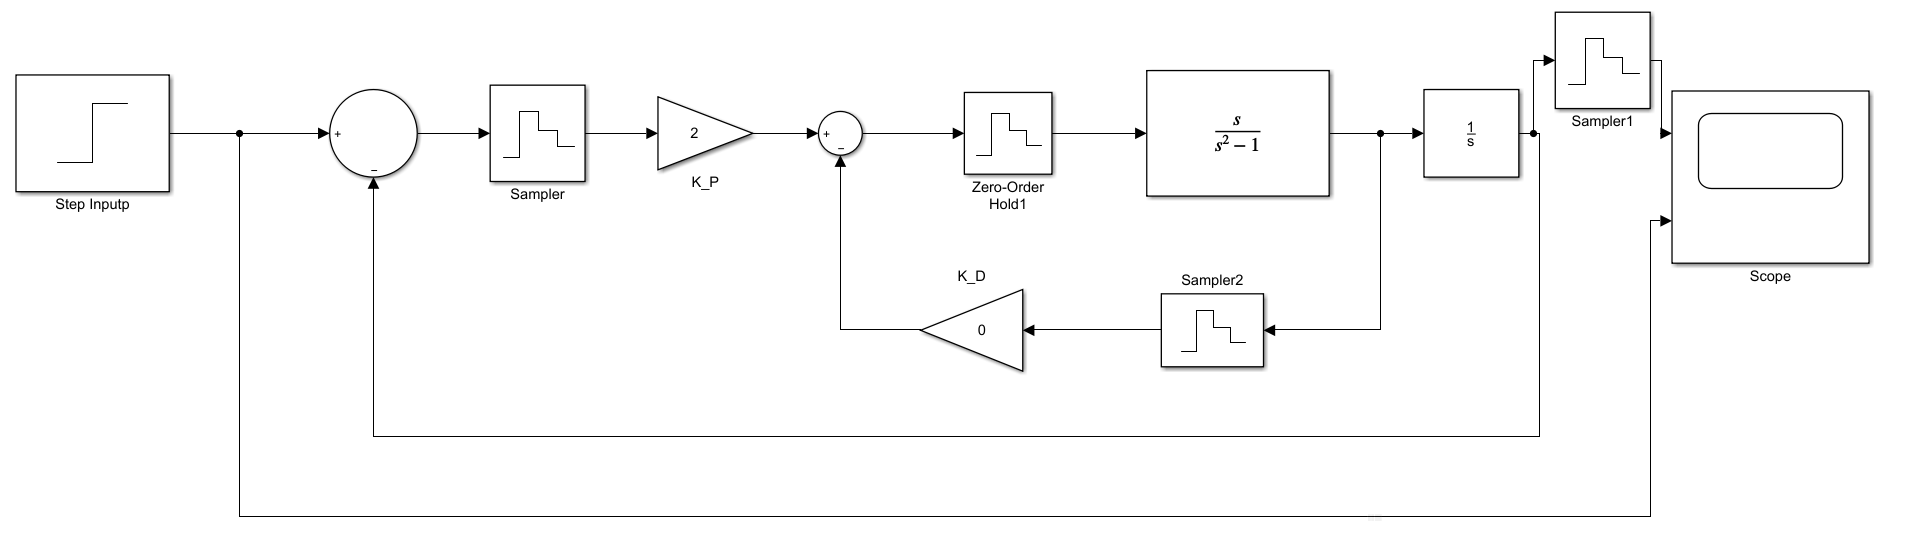
\includegraphics[width=1.0\unitlength]{images/simu3}
 				\caption{\label{fig:simu1} Simulink Model for the given system with $K_P=2$ and $K_D=0$}
 			\end{figure}
 		
 		The \textit{Figures~\ref{fig:s1}\ ,\ \ref{fig:s2}} shows the step response of the given system  with simulink. The Simulink model can be seen at \textit{Figure~\ref{fig:simu1}}.
 		
		 \begin{figure}[H]
 			\setlength{\unitlength}{\textwidth} 
 			\centering
 			\begin{subfigure}{.5\textwidth}
   				\centering
   				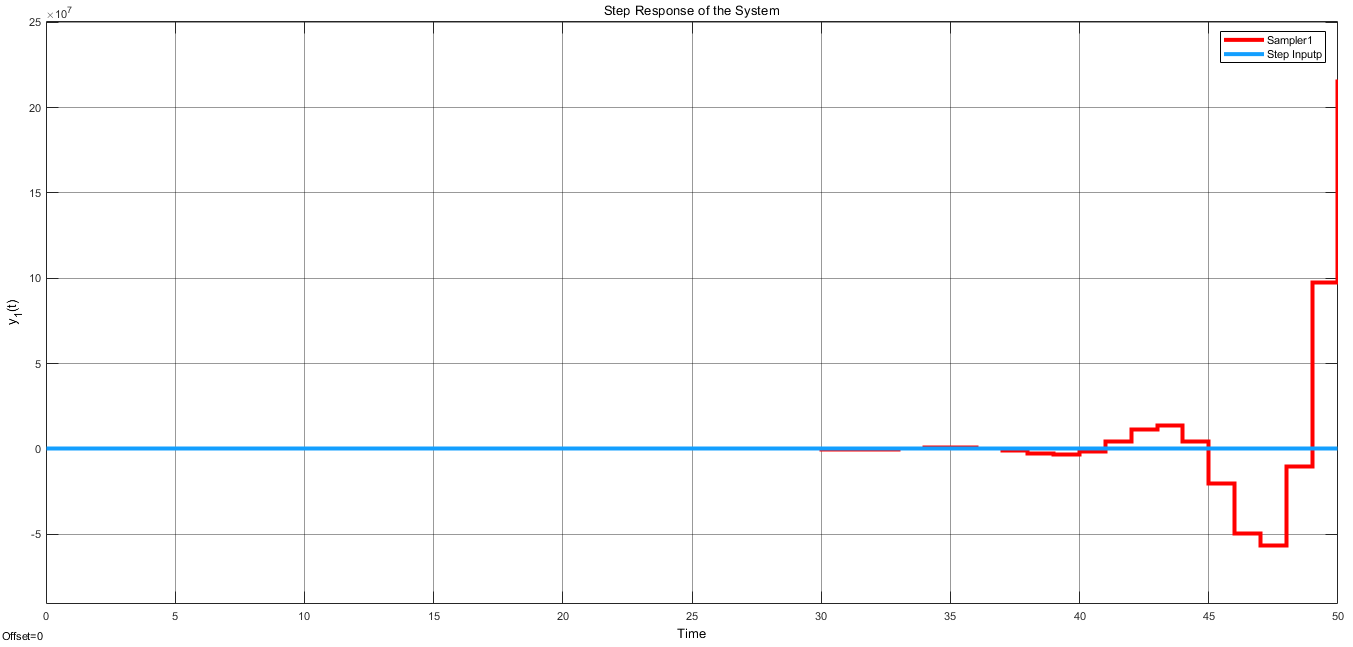
\includegraphics[width=0.48\unitlength]{images/1c}
   				\caption{\label{fig:s1} Step Response of the $y_1[k]$ till $k=50$ with Simulink}
 			\end{subfigure}%
 			\begin{subfigure}{.5\textwidth}
   				\centering
 				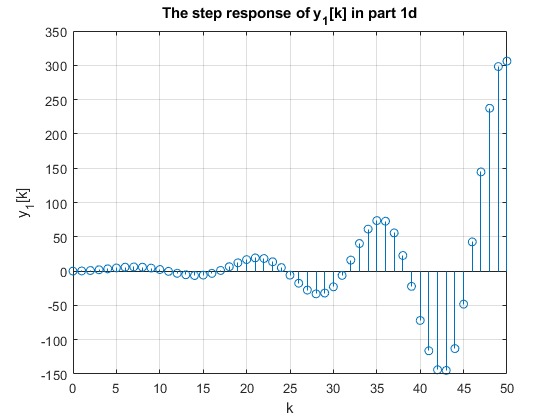
\includegraphics[width=0.48\unitlength]{images/1ca}
   				\caption{\label{fig:s2} Step Response of the $y_1[k]$ till $k=50$ }
 			\end{subfigure}
			 %\caption{\label{fig:step} Step Responses of the given system with varying end times  }	
		 \end{figure}
		 
		  \begin{figure}[H]
 			\setlength{\unitlength}{\textwidth} 
 			\centering
 			\begin{subfigure}{.5\textwidth}
   				\centering
   				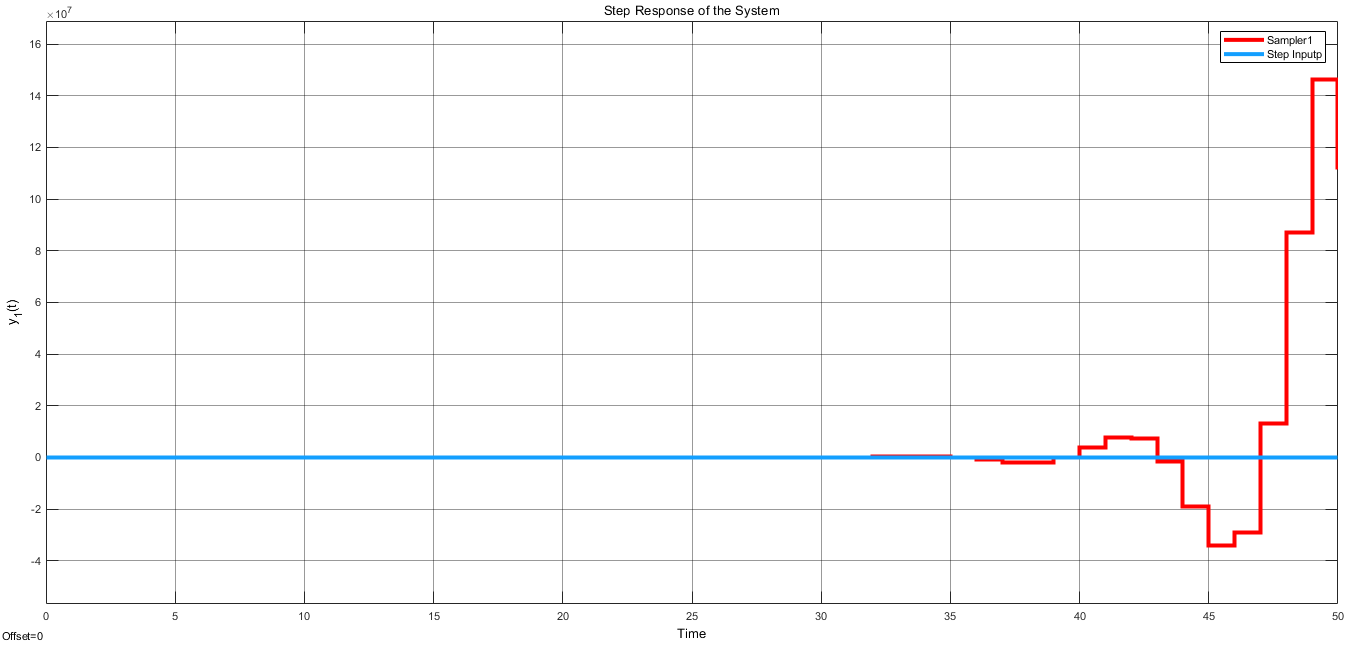
\includegraphics[width=0.48\unitlength]{images/1cb}
   				\caption{\label{fig:s1} Step Response of the $y_2[k]$ till $k=50$ with Simulink}
 			\end{subfigure}%
 			\begin{subfigure}{.5\textwidth}
   				\centering
 				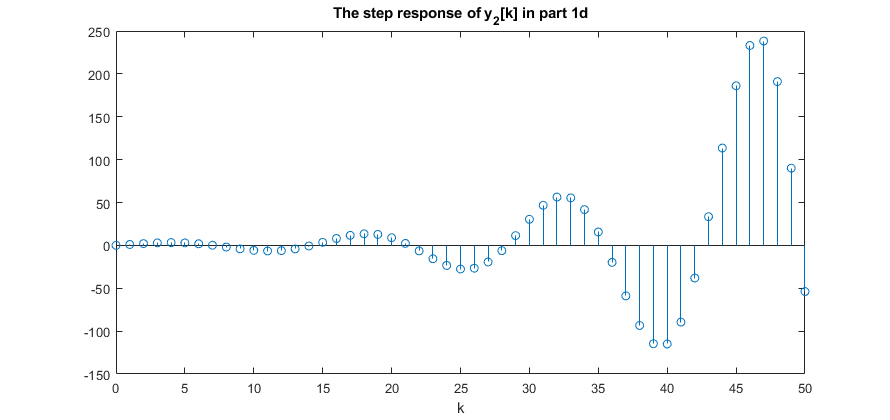
\includegraphics[width=0.48\unitlength]{images/1cba}
   				\caption{\label{fig:s2} Step Response of the $y_2[k]$ till $k=50$ }
 			\end{subfigure}
			 %\caption{\label{fig:step} Step Responses of the given system with varying end times  }	
		 \end{figure}
		 
		 It can be observed from the figures also that the system shows very unstable behaviour with given $K_p$ value.
		 
		  
 		\newpage
 		\item Let us analyse the system now with a $K_d \neq 0$
 		
 		\begin{equation*}
			\begin{split}		
				 E(s) &= R(s) - Y_1(s)  \\
				 E^*(s) &= R^*(s) - Y_1^*(s) 
				 \\[0.3cm]  \hline \\[-0.3cm]		 
				 Y_2(s) &= \left[ E^*(s) K_p - K_D Y_2^*(s)\right]G_X(s)  \\
				 Y^*_2(s) &= \left[ E^*(s) K_p - K_D Y_2^*(s)\right]G_X^*(s)  \\[0.3cm]
				 \frac{Y_2^*(s)}{E^*(s)}&=\frac{K_p G_X^*(s)}{1+K_D G_X^*(s)}  
				 \\[0.3cm]  \hline \\[-0.3cm]
				 Y_1(s) &= \left[ E^*(s) K_p - K_D Y_2^*(s)\right]G_Y(s)  \\
				 Y^*_1(s) &= \left[ E^*(s) K_p - K_D Y_2^*(s)\right]G_Y^*(s)  \\	
				  &= E^*(s)\left[ K_p - K_D \frac{K_p G_X^*(s)}{1+K_D G_X^*(s)} \right] G_Y^*(s) \\
				  &= E^*(s)\left[  \frac{K_p}{1+K_D G_X^*(s)} \right] G_Y^*(s) \\[0.3cm]
				 \frac{Y_1^*(s)}{E^*(s)}&= \frac{K_P G_Y^*(s)}{1+K_D G_X^*(s)}
				 	\\[0.3cm]  \hline \\[-0.3cm]		 
				 E^*(s) &= R^*(s) - E^*(s) \frac{K_P G_Y^*(s)}{1+K_D G_X^*(s)} \\[0.3cm]
				 R^*(s) &= E^*(s) \left( 1+ \frac{K_P G_Y^*(s)}{1+K_D G_X^*(s)}\right) \\[0.3cm]
				 \frac{E^*(s)}{R^*(s)}&=\cfrac{1}{1+ \cfrac{K_P G_Y^*(s)}{1+K_D G_X^*(s)}} \\	  
				 &= \frac{1+K_D G_X^*(s)}{1+K_D G_X^*(s)+K_P G_Y^*(s)}  \\[0.3cm]  \hline \\[-0.3cm]	
				 \frac{Y_1^*(s)}{R^*(s)} &=  \ \frac{Y_1^*(s)}{E^*(s)} \frac{E^*(s)}{R^*(s)}  = \frac{K_P G_Y^*(s)}{1+K_D G_X^*(s)+K_P G_Y^*(s)}  
				 \\[0.3cm]  \hline \\[-0.3cm]	
				 \frac{Y_2^*(s)}{R^*(s)} &=  \ \frac{Y_2^*(s)}{E^*(s)} \frac{E^*(s)}{R^*(s)}  = \frac{K_p G_X^*(s)}{1+K_D G_X^*(s)+K_P G_Y^*(s)} 
			\end{split}
		\end{equation*}
		

		Thus, with $s=\frac{1}{T}ln(z)$
		$$\boxed{ \frac{Y_1(z)}{R(z)} = \frac{K_P G_Y(z)}{1+K_D G_X(z)+K_P G_Y(z)} }$$
		
		$$\boxed{ \frac{Y_2(z)}{R(z)} = \frac{K_p G_X(z)}{1+K_D G_X(z)+K_P G_Y(z)}  }$$
		
		Remember that, the $G_x(z)$ and $G_Y(z)$ were found earlier as
		
		$$\boxed  { G_Y(z)\approx \frac{0.1275(z+1)}{z^2-2.255z+1} }$$		
	
		$$\boxed  { G_X(z)\approx \frac{0.52  \left(z-1 \right) }{z^2-2.255z+1 } }$$
		
		\begin{equation*}
			\begin{split}
				\frac{Y_1(z)}{R(z)} &= \frac{K_P G_Y(z)}{1+K_D G_X(z)+K_P G_Y(z)} \\[0.3cm]
				&= \cfrac{K_P \left(\cfrac{0.1275(z+1)}{z^2-2.255z+1}\right) }{1+K_D \left(\cfrac{0.52  \left(z-1 \right) }{z^2-2.255z+1 }\right)+K_P \left(\cfrac{0.1275(z+1)}{z^2-2.255z+1}\right)}  \\[0.3cm]
				&=\frac{0.1275K_p(z+1)}{z^2-2.255z+1+0.52K_D(z-1)+0.1275K_P(z+1)}
			\end{split}
		\end{equation*}
		
		$$\boxed{ \cfrac{Y_1(z)}{R(z)} =\cfrac{0.1275K_p(z+1)}{z^2+(0.52K_D+0.1275K_P-2.255)z+(1-0.52K_D+0.1275K_P)} }$$
		
		\begin{equation*}
			\begin{split}
				\frac{Y_2(z)}{R(z)} &= \frac{K_p G_X(z)}{1+K_D G_X(z)+K_P G_Y(z)}  \\[0.3cm]
				&= \frac{K_p \left(\cfrac{0.52  \left(z-1 \right) }{z^2-2.255z+1 }\right)}{1+K_D \left(\cfrac{0.52  \left(z-1 \right) }{z^2-2.255z+1 }\right)+K_P \left(\cfrac{0.1275(z+1)}{z^2-2.255z+1}\right)}  \\[0.3cm]
				&=\frac{0.52K_p(z-1)}{z^2-2.255z+1+0.52K_D(z-1)+0.1275K_P(z+1)}  \\[0.3cm]
			\end{split}
		\end{equation*}
		
		$$\boxed{ \cfrac{Y_2(z)}{R(z)} =\cfrac{0.52K_p(z-1)}{z^2+(0.52K_D+0.1275K_P-2.255)z+(1-0.52K_D+0.1275K_P)} }$$
		
		\item Let us use Jury stability test again
		
		\begin{equation*}
			\begin{split}
				D(z)&=z^2+(0.52K_D+0.1275K_P-2.255)z+(1-0.52K_D+0.1275K_P)  \\
				&=z^2+(-2+0.52K_D)z+(1.255-0.52K_D) \\
			\end{split}
		\end{equation*}
		
			With coefficients, 
		$$ \boxed{a_0=1} \ , \ \boxed{a_1=-2+0.52K_D} \ ,\ \boxed{a_2=1.255-0.52K_D} $$		
		The characteristic polynomial $D(z)$ should satisfy the following conditions according to Jury stability conditions;
		\begin{itemize}
			\item $a_0\ >\ |a_2| $ \\
			$$ 1\ >\ 1.255-0.52K_D > -1 $$
			$$\boxed{ 4.27 > K_D > 0.49 }$$
			\item $D(1)>0$ \\
			$$ 1-2+0.52K_D+1.255-0.52K_D > 0$$
			$$ \boxed{ 0.255>0} $$
			\item $D(-1)>0$ \\
			$$ 1+2-0.52K_D+1.255-0.52K_D > 0$$
			$$ 4.255-1.04K_D>0 $$
			$$\boxed{ 4.06>K_D }$$				
		\end{itemize}
		It can be concluded that  $K_D$ should satisfy the following
		
		$$\boxed{ 4.06 > K_D > 0.49 }$$
		
		
		
		\item Let us choose \textbf{$K_D=2$} 
		
			$$\cfrac{Y_1(z)}{R(z)} =\cfrac{0.255(z+1)}{z^2-0.93+0.255}$$
			
			$$\boxed{ Y_1(z)= \cfrac{0.255z(z+1)}{(z^2-0.93+0.255)(z-1)} }$$	
			
				
			$$ \cfrac{Y_2(z)}{R(z)} =\cfrac{1.04(z-1)}{z^2-0.93+0.255}$$
			
			$$\boxed{ Y_2(z)= \cfrac{1.04z}{z^2-0.93+0.255} }$$	
		
		
		\item The \textit{Figure\ \ref{fig:stepy1b}} shows the step responses of $y_1(t)$ and $y_2(t)$ respectively. The source code for that operation can be seen at \textbf{Appendix~\ref{appendix}}.
		 
		
		 
		  \begin{figure}[H]
		 	\center
		 	\setlength{\unitlength}{\textwidth} 
		 	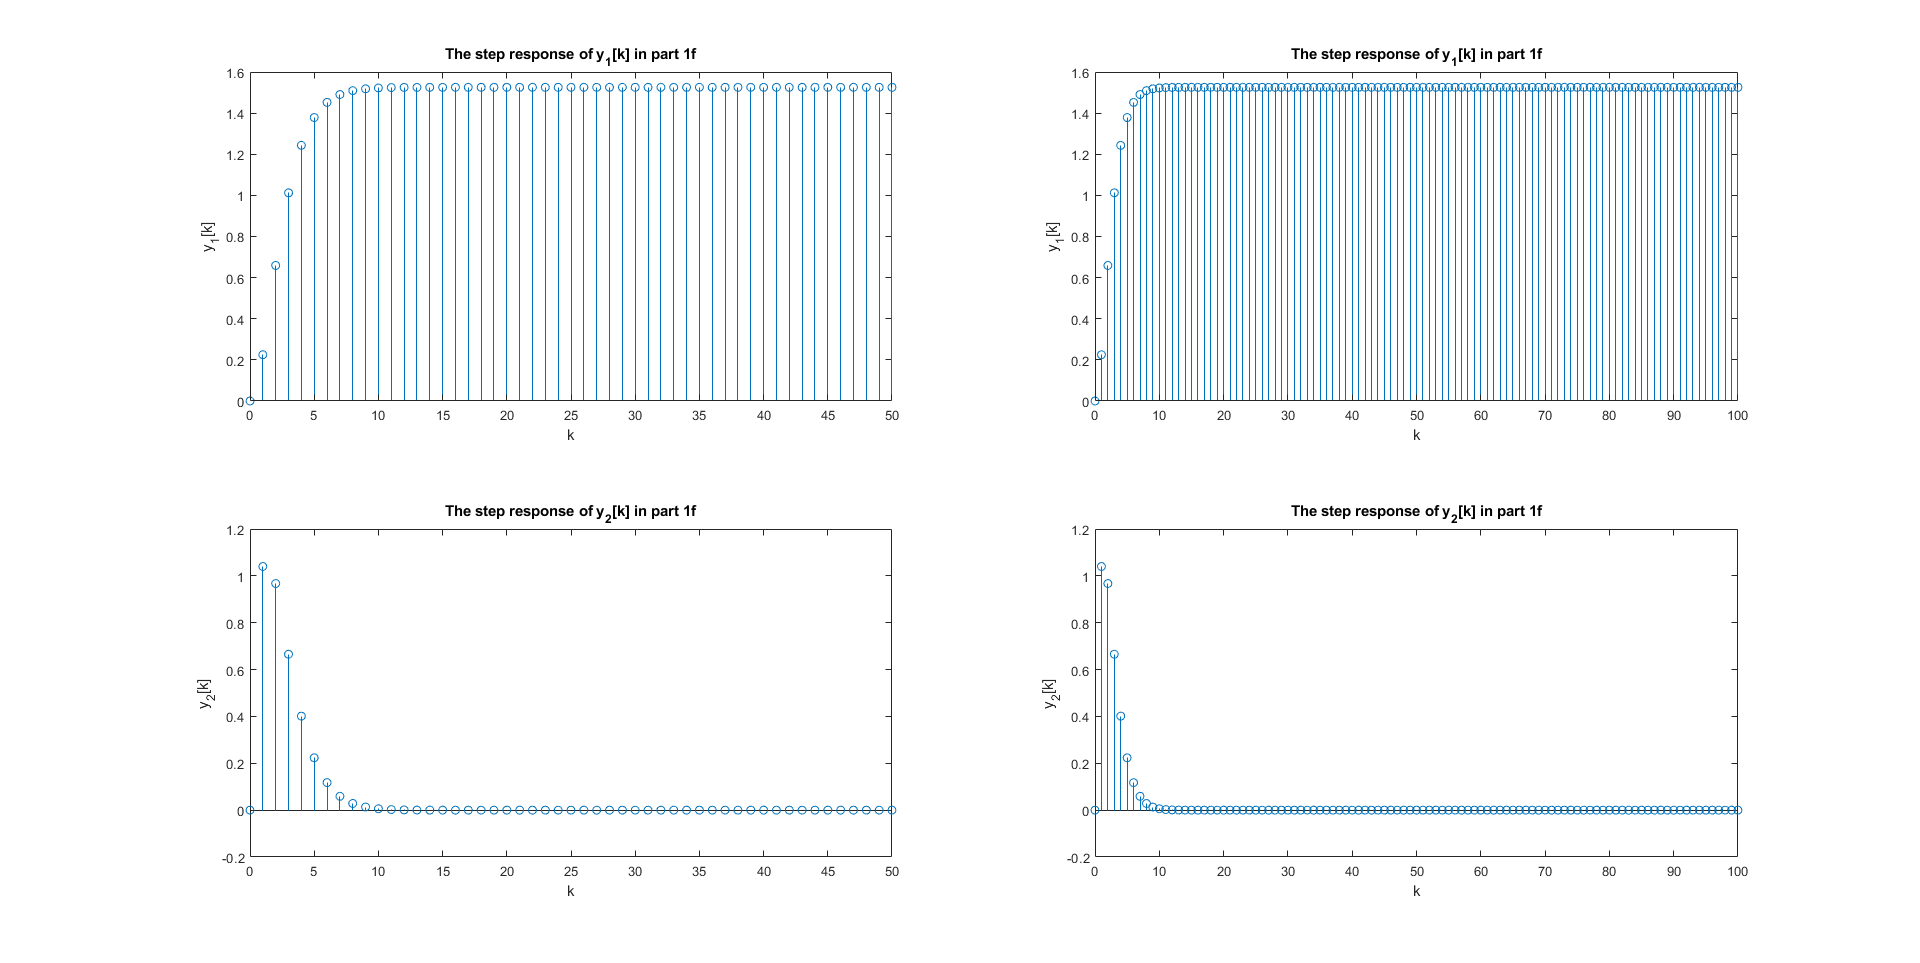
\includegraphics[width=1.0\unitlength]{images/1f}
		 	\caption{\label{fig:stepy1b} Step Response for the $y_1(t)$ with $K_P=2$ and $K_D=2$}
		 \end{figure}
	 	
	 	
		 
		\begin{figure}[H]
			\center
			\setlength{\unitlength}{\textwidth} 
			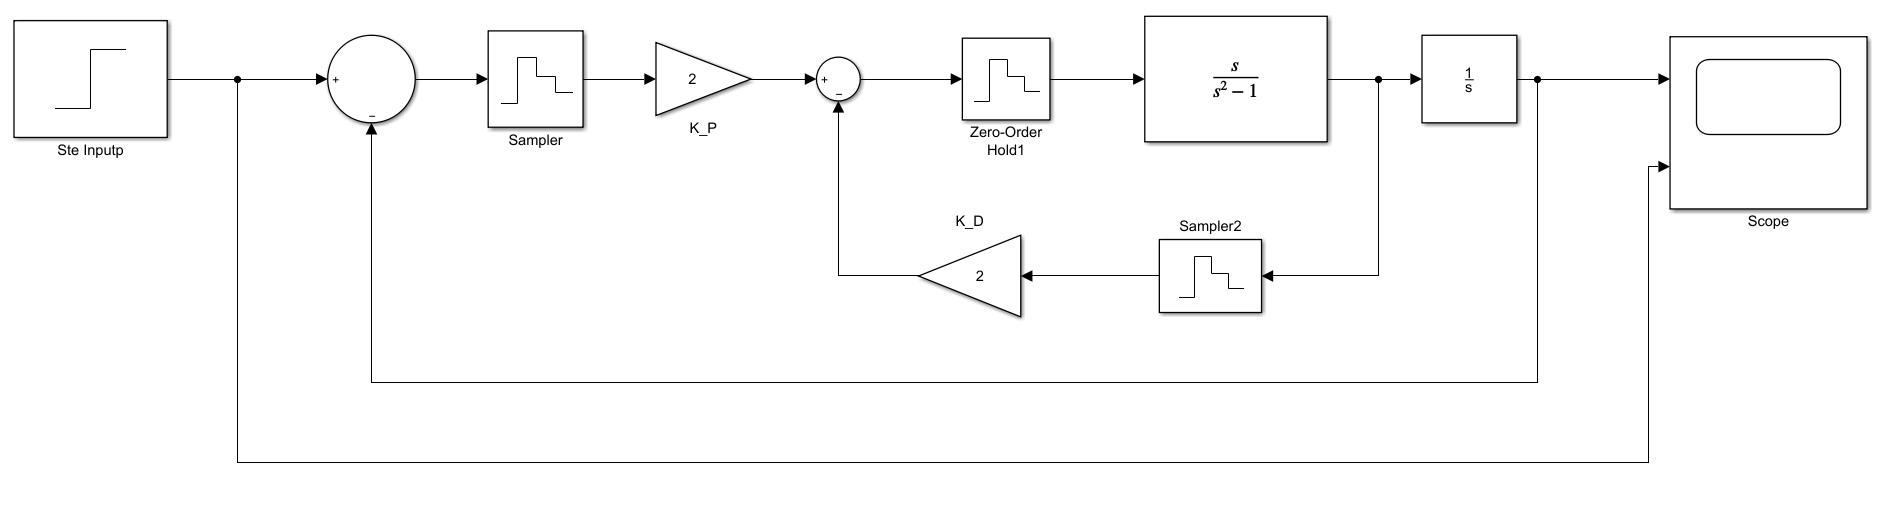
\includegraphics[width=1.0\unitlength]{images/simu2}
			\caption{\label{fig:simu2} Simulink Model for the given system with $K_P=2$ and $K_D=2$}
		\end{figure}
		
		The \textit{Figure~\ref{fig:step2}} shows the step response of the given system  with simulink. The Simulink model can be seen at \textit{Figure~\ref{fig:simu2}}. Although the System acts very stable at the very beginning of the operation, the step response goes further stability limits as $t \to \infty $ as can be seen from the \textit{Figure~\ref{fig:sb5}}. 
		
		\begin{figure}[H]
			\setlength{\unitlength}{\textwidth} 
			\centering
			\begin{subfigure}{.5\textwidth}
				\centering
				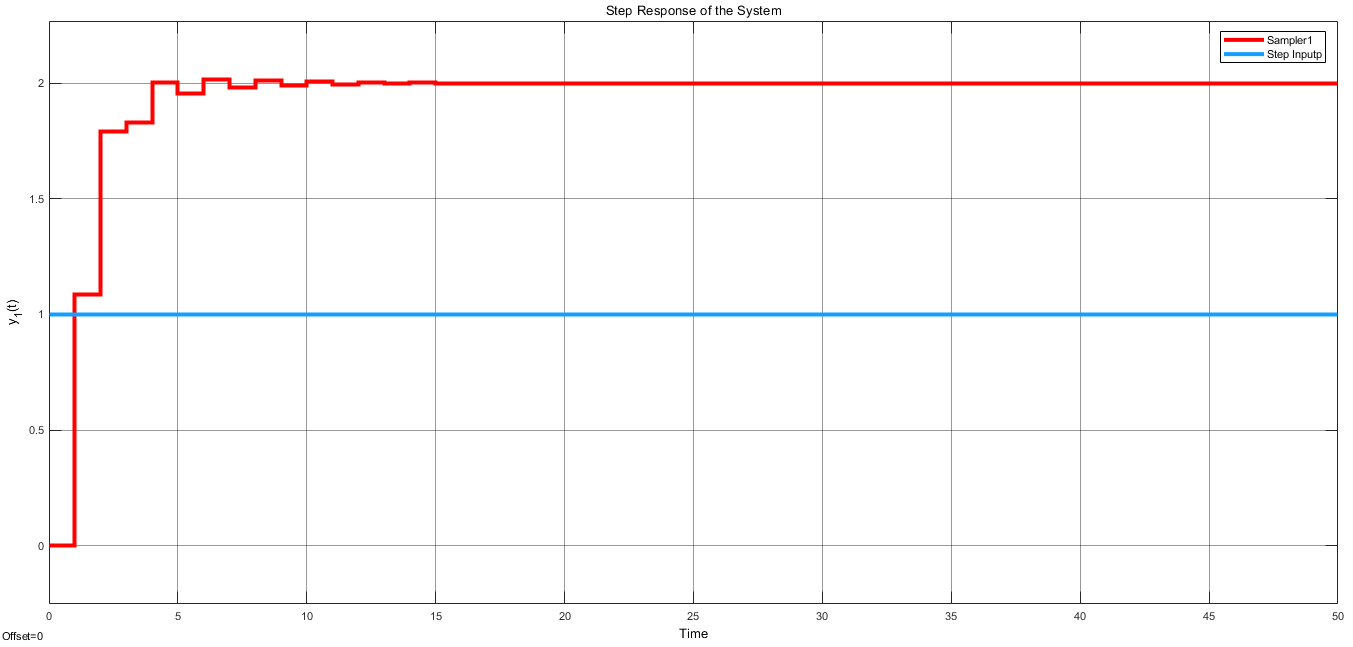
\includegraphics[width=0.48\unitlength]{images/1g}
				\caption{\label{fig:sb1} Step Response of the $y_1[k]$ till $k=50$ with Simulink }
			\end{subfigure}%
			\begin{subfigure}{.5\textwidth}
				\centering
				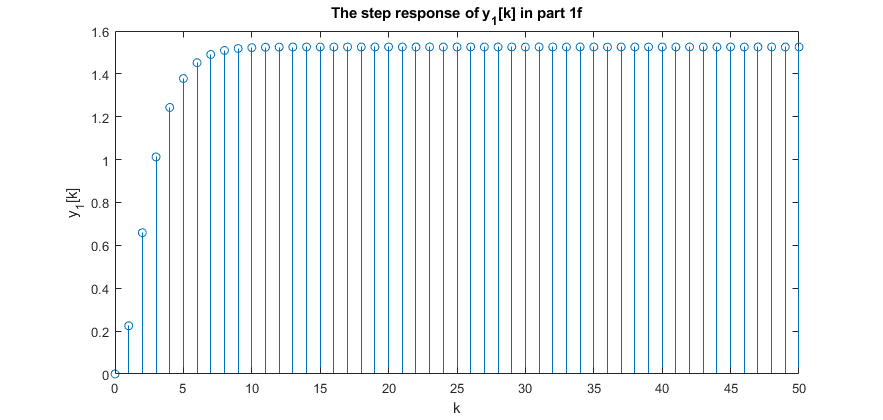
\includegraphics[width=0.48\unitlength]{images/1fa}
				\caption{\label{fig:sb2} Step Response of the $y_1[k]$ till $k=50$ }
			\end{subfigure}
			%\caption{\label{fig:step2} Step Responses of the given system with varying end times  }	
		\end{figure}
		
		\begin{figure}[H]
			\setlength{\unitlength}{\textwidth} 
			\centering
			\begin{subfigure}{.5\textwidth}
				\centering
				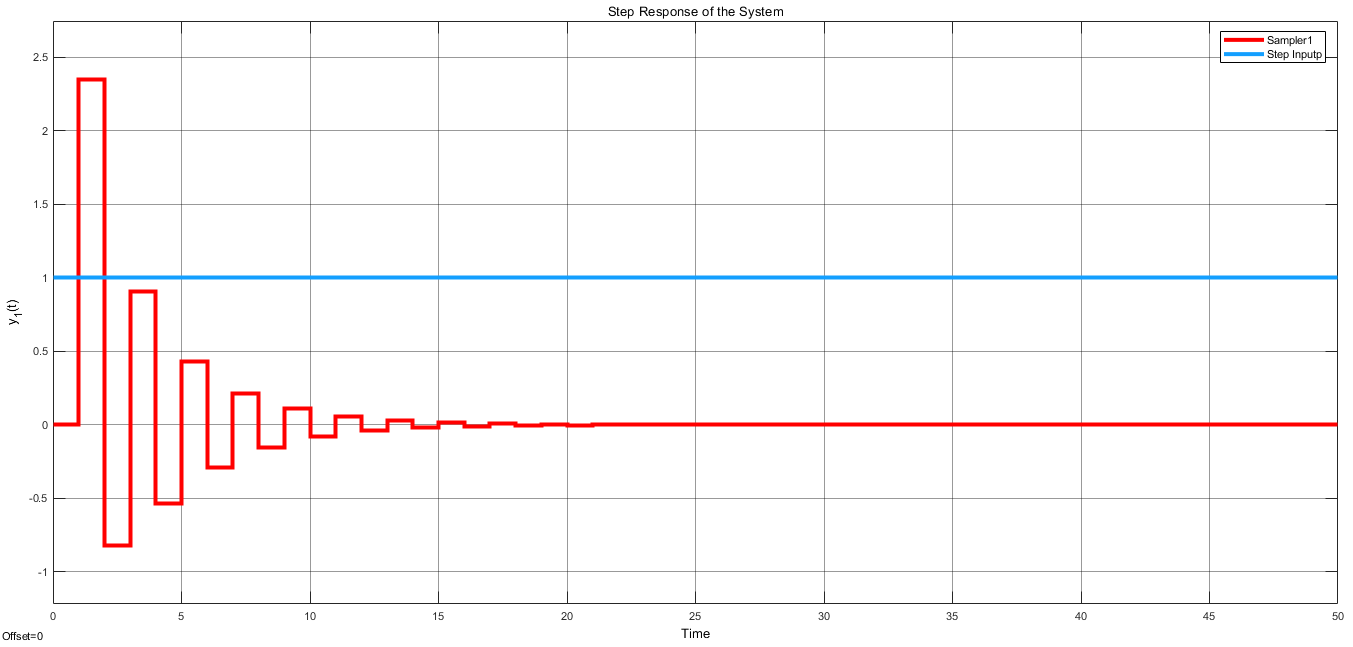
\includegraphics[width=0.48\unitlength]{images/1gb}
				\caption{\label{fig:sb1} Step Response of the $y_2[k]$ till $k=50$ with Simulink }
			\end{subfigure}%
			\begin{subfigure}{.5\textwidth}
				\centering
				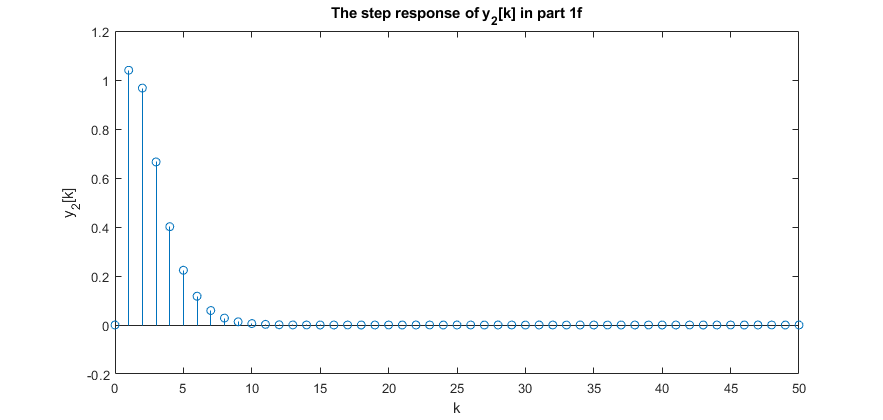
\includegraphics[width=0.48\unitlength]{images/1gba}
				\caption{\label{fig:sb2} Step Response of the $y_2[k]$ till $k=50$ }
			\end{subfigure}
			%\caption{\label{fig:step2} Step Responses of the given system with varying end times  }	
		\end{figure}
	
	 	
	\end{enumerate}
\end{enumerate}
	
%		\newpage
%\begin{appendices}
%	\section{Source Code For Question 2}
%		\lstinputlisting[language=Matlab]{q2.m} \-\\[1cm]

%		\lstinputlisting[language=Matlab]{mydelta.m} \-\\[1cm]
%		\newpage
%	\section{Source Code For Question 3}
%		\lstinputlisting[language=Matlab]{q3.m} \-\\[1cm]
%	\section{Source Code For Question 4}
%		\lstinputlisting[language=Matlab]{q4.m} \-\\[1cm]
%				\lstinputlisting[language=Matlab,firstline=33, lastline=34]{q13.m} \-\\[1cm]
%\end{appendices}
				
\newpage
\begin{appendices}
\section{Source Code for Matlab Part}\label{appendix}
	%%	\lstinputlisting[language=Matlab,firstline=33, lastline=34]{q13.m} \-\\[1cm]		
\lstinputlisting[language=Matlab]{Q1.m} 






\end{appendices}


\end{document}

%----samples------
%\begin{itemize}
%\item Item
%\item Item
%\end{itemize}

%\begin{figure}[H]
%\center
%\setlength{\unitlength}{\textwidth} 
%\includegraphics[width=0.7\unitlength]{images/logo1}
%\caption{\label{fig:logo}Logo }
%\end{figure}

%\begin{figure}[H]
%	\setlength{\unitlength}{\textwidth} 
%	\centering
%	\begin{subfigure}{.5\textwidth}
%  		\centering
%  		\includegraphics[width=0.48\unitlength]{images/logo1}
%  		\caption{\label{fig:logo1}Logo1 }
%	\end{subfigure}%
%	\begin{subfigure}{.5\textwidth}
%  		\centering
%		\includegraphics[width=0.48\unitlength]{images/logo2}
%  		\caption{\label{fig:logo2}Logo2}
%	\end{subfigure}
%\caption{\label{fig:calisandegree} Small Logos   }
%\end{figure}
	
%\begin{table}[H]
%  \centering
% 
%    \begin{tabular}{c|c|c}
%       $$A$$ & $$B$$ & $$C$$ \\ \hline
%       1 & 2 & 3  \\ \hline
%       2 & 3 & 4  \\ \hline
%       3 & 4 & 5  \\ \hline
%       4 & 5 & 6  
%      
%  \end{tabular}
%  \caption{table}
%  \label{tab:table}
%\end{table}
	
%\begin{table}[H]
%  \centering
% 
%    \begin{tabular}{c|c|c}
%       \backslashbox{$A$}{$a$} & $$\specialcell{ Average deviation \\ after subtracting out the  \\ frequency error }$$ & $$C$$ \\ \hline
%       \multirow{2}{*}{1} & 2 & 3  \\ \cline{2-3}
%        & 3 & 4  \\ \hline
%       3 & \multicolumn{2}{c}{4}  \\ \hline
%       4 & 5 & 6  
%      
%  \end{tabular}
%  \caption{table}
%  \label{tab:table}
%\end{table}
%-----end of samples-----